\documentclass[10pt,a4paper]{article}
\usepackage[margin=2cm]{geometry}
\usepackage{amsmath,iftex}
\ifPDFTeX\usepackage[T1]{fontenc}\usepackage[utf8]{inputenc}\else\usepackage{unicode-math}\fi
\usepackage{lmodern,graphicx,booktabs,array,longtable,microtype,parskip,xcolor}
\usepackage{hyperref}\usepackage{xurl}
\hypersetup{hidelinks,pdftitle={Contextual Bandits for News Recommendation under Changing User Preferences},pdfauthor={DSC6007 Group 14}}
\setlength{\emergencystretch}{3em}
\newcommand{\E}{\mathrm{E}}
\begin{document}
\begin{center}
{\Large\bfseries Contextual Bandits for News Recommendation\\under Changing User Preferences}\par\vspace{6pt}
{\large Chronological Yahoo Replay and Controlled Drift Experiments}\par\vspace{5pt}
\textbf{DSC6007 Dynamic Programming and Reinforcement Learning --- Group 14}\\
LI Yizhuo \quad ZHANG Tianyi \quad GOU Zhijie \quad AN Yuxian \quad XIAO Yuhang\\
Semester A 2026
\end{center}

\subsection*{Abstract}
News recommendation must personalise article selection from partial click
feedback while adapting to changing interests. We implement both Li et al.
(2010) estimators: LinUCB (disjoint), with one ridge fit per article, and
LinUCB (hybrid), with a per-article term plus a coefficient shared across
36 user--article interaction features, estimated jointly by block-matrix
inversion. A chronological Yahoo! R6A replay (100,000 events) and a
controlled drift simulator evaluate seven policies, including the paper's
context-free $\epsilon$-greedy and an explicitly named contextual-greedy
variant. On Yahoo, Hybrid has 788 matched events and 3.807\% replay CTR
versus 780 and 3.846\% for Disjoint; policy-dependent matched sets preclude
a reliable ranking. A fixed-test sparse-data diagnostic (100/10/5/1\%
warmup, plus a 50-article pool) probes the paper's sparse-learning claim and
does not reproduce that advantage on this log.
Ten-seed simulations favour a 300-round window under specified changes;
20 independent seeds and an intercept ablation test that result. Forgetting
can help in the tested drift worlds, but neither replay nor simulation
establishes an online gain. Settings, hashes and a frozen Python 3.13.2
lockfile accompany the report.

\section{Introduction}
\subsection{Motivation and research questions}
A news service sees a user and candidate articles, shows one, and observes
a click; rewards for unshown items stay unobserved. Contextual bandits
address this exploration--exploitation problem \cite{li2010}, but
personalisation alone fails when interests move: using all past feedback
may adapt slowly, while discarding old data trades tracking against
estimation precision. We combine a chronological evaluation on real logged
feedback with a simulator that deliberately changes preferences: Yahoo
tests recommendation behaviour on a logged slice, and controlled drift
tests adaptation against known counterfactual means. We ask (Q1) what the
policies achieve under the Yahoo protocol, (Q2) whether a recent-data
window improves tracking under known change, and (Q3) how feature
specification and window size affect that conclusion.

\subsection{Course connection, related work and contributions}
The project applies contextual bandits, optimistic exploration, ridge
estimation and non-stationary sequential decisions. Li et al.
\cite{li2010} define Disjoint and Hybrid LinUCB; Li et al. \cite{li2011}
give replay evaluation conditions. Cheung et al. \cite{cheung2019}, Russac
et al. \cite{russac2019} and Zhao et al. \cite{zhao2020} study windows,
discounting and restarts; our window rule is not their algorithm or
guarantee. We do not transfer a regret bound past the cautions of Faury et
al. \cite{faury2021}. Contributions: faithful Algorithms 1--2 checked
against the joint ridge solution; a chronological Yahoo-plus-drift design;
and an independent simulation extension. Negative results are retained;
no new theorem or online gain is claimed.

\section{Methods and theoretical interpretation}
\subsection{Bandit formulation and rewards}
At event $t$, observe user $u_t$ and candidates $\mathcal A_t$; choose
$a_t\in\mathcal A_t$ and see $r_t\in\{0,1\}$ (click). The objective is
$\E[\sum_t r_t]$. A Yahoo event also contains the logger action $\ell_t$
and only its reward: we update only when $a_t=\ell_t$ and never label an
unshown item as a non-click. In simulation, with known means $\mu_t(a)$,
we measure dynamic pseudo-regret
\begin{equation}
R_T=\sum_{t=1}^T\left[\max_{a\in\mathcal A_t}\mu_t(a)-\mu_t(a_t)\right].
\label{eq:regret}
\end{equation}
The evaluator knows these means; policies see only chosen rewards. Yahoo
has no counterfactual labels, so true regret is not computed there.

\subsection{Disjoint LinUCB}
Each article $a$ has its own ridge fit on the six-dimensional user context
$x_{t,a}$:
\begin{equation}
A_{a,t}=\lambda I+\sum_{i\in\mathcal I_{a,t}}x_ix_i^\top,\quad
b_{a,t}=\sum_{i\in\mathcal I_{a,t}}r_ix_i,\quad
\hat\theta_{a,t}=A_{a,t}^{-1}b_{a,t}.
\label{eq:ridge}
\end{equation}
$\mathcal I_{a,t}$ holds only matched feedback. With $\lambda=1$, LinUCB chooses
\begin{equation}
a_t=\arg\max_{a\in\mathcal A_t}
\left[x_{t,a}^\top\hat\theta_{a,t}
+\alpha\sqrt{x_{t,a}^\top A_{a,t}^{-1}x_{t,a}}\right].
\label{eq:ucb}
\end{equation}
The confidence reading needs a bounded, correctly specified linear mean
and sub-Gaussian noise; our validation-selected $\alpha$ is heuristic,
not calibrated coverage.

\subsection{Hybrid LinUCB (Li et al. 2010, Algorithm 2)}
The Hybrid model adds a term shared across all articles:
\begin{equation}
\E[r_{t,a}\mid x_{t,a},z_{t,a}]
= z_{t,a}^\top\beta^* + x_{t,a}^\top\theta_a^*,
\label{eq:hybridmean}
\end{equation}
with $x_{t,a}\in\mathbf R^6$ the user context and $\beta^*$ shared across
articles. Following Li et al. (2010, Sec.~5.2.2), the shared feature is
$z_{t,a}=\mathrm{vec}(u_t v_a^\top)\in\mathbf R^{36}$, carrying
user--article interaction information; $x_{t,a}$ carries user information
only. Both parameter sets come from one joint ridge system. Maintain
$A_a=I+\sum xx^\top$, $B_a=\sum xz^\top$, $b_a=\sum rx$ per arm and
$A_0=I+\sum zz^\top$, $b_0=\sum rz$ globally. Define the Schur complement
\begin{equation}
S=A_0-\sum_a B_a^\top A_a^{-1}B_a .
\label{eq:schur}
\end{equation}
Then the shared and per-arm estimates are
\begin{equation}
\hat\beta=S^{-1}\!\left(b_0-\sum_a B_a^\top A_a^{-1}b_a\right),\qquad
\hat\theta_a=A_a^{-1}\left(b_a-B_a\hat\beta\right).
\label{eq:hybridfit}
\end{equation}
This is the joint least-squares solution. The UCB score uses the predictive
variance of $x^\top\hat\theta_a+z^\top\hat\beta$,
\begin{equation}
s_{t,a}=z^\top S^{-1}z-2z^\top S^{-1}B_a^\top A_a^{-1}x
+x^\top A_a^{-1}x+x^\top A_a^{-1}B_a S^{-1}B_a^\top A_a^{-1}x,
\label{eq:hybridvar}
\end{equation}
or equivalently $s_{t,a}=x^\top A_a^{-1}x+(z-B_a^\top A_a^{-1}x)^\top
S^{-1}(z-B_a^\top A_a^{-1}x)$; the score is
$z^\top\hat\beta+x^\top\hat\theta_a+\alpha\sqrt{s_{t,a}}$. The last term
in Eq.~\eqref{eq:hybridvar} is the cross-arm uncertainty from sharing
$\beta$; it distinguishes Hybrid from a widened Disjoint UCB. Updates are
incremental on matched feedback, with dense recomputation of $S^{-1}$ when
needed. Tests check the joint solve and the literal Algorithm 2 variance.

\paragraph{Feature fidelity to the source paper.}
Li et al. (2010, Sec.~5.2.2) binarise and unit-normalise the raw
categorical vectors before a conjoint reduction to six dimensions. The
R6A files expose only the resulting six user and six article coordinates,
not the upstream projection. We therefore build $z_{t,a}$ from the
supplied six-vectors as-is; the paper's unit-length step precedes
dimensionality reduction and does not apply to the final six features.
This is the one deliberate preprocessing deviation; the 36-dimensional
shared structure is preserved.

\paragraph{Disambiguating $x_{t,a}$, and two distinct greedy baselines.}
Li et al. (2010, Sec.~5.2.2) state that $x_{t,a}$ is ``exactly the
six-dimensional feature constructed as above for user $u_t$'' and
``contains user information only'', while $z_{t,a}=\mathrm{vec}(u_t
v_a^\top)$ is separate. Concatenating article coordinates into $x$ would
make it twelve-dimensional, contradict the source and double-count article
information already in $z$. Our \texttt{context()} map is faithful; no
change was needed after this audit. We report two greedy comparators.
\emph{contextual greedy} uses the disjoint ridge mean with probability
$1-\epsilon$, a uniform candidate otherwise, and zero UCB width (the
variant carried over from the original code). \emph{$\epsilon$-greedy
(context-free)} follows Li et al. (2010, Secs.~2.2, 5.3): it ignores all
features, keeps empirical per-article click means, and explores uniformly
with probability $\epsilon$. Uniform Random is a third reference. Rewards
remain binary; no shaped non-click penalty is used.

\subsection{Window adaptation and the bias--precision trade-off}
For Yahoo, Window LinUCB retains matched observations with log index
$t-W\le i<t$; the clock advances on \emph{every} logged event, so
$W=5{,}000$ counts log events, not feedback updates or seconds. In
simulation every round yields feedback, so its 300-round window uses a
different unit.

For one arm, let $r_i=x_i^\top\theta_i+e_i$. An exact identity is
\begin{equation}
\hat\theta_t-\theta_t=A_t^{-1}\left[
\sum_{i\in\mathcal I_t}x_ix_i^\top(\theta_i-\theta_t)
+\sum_{i\in\mathcal I_t}x_ie_i-\lambda\theta_t\right].
\label{eq:drift}
\end{equation}
\emph{Derivation.} Substitute into Eq.~\eqref{eq:ridge}, subtract
$A_t^{-1}A_t\theta_t$, and collect coefficient-change, residual and ridge
terms. The identity is algebraic and holds under misspecification.

Under a stationary mean the first term vanishes; under drift stale data
can bias the fit while a short window also reduces precision. This is a
conditional motivation, not a theorem that shorter always wins. Rank-one
updates insert observations and inverse downdates remove expired ones;
scoring and updates cost $O(d^2)$, with a dense $O(d^3)$ fallback. State
holds $K$ inverse matrices and a queue of retained matches, not
linear-in-dimension memory.

\subsection{Replay, predictive metrics and off-policy checks}
The Yahoo metrics are
\[
\widehat{\mathrm{CTR}}_{\rm replay}=
\frac{\sum_t\mathbf1[a_t=\ell_t]r_t}{\sum_t\mathbf1[a_t=\ell_t]},
\qquad \mathrm{match\ rate}=\frac{\#\{a_t=\ell_t\}}{\#\mathrm{log\ events}}.
\]
Replay can evaluate deterministic policies under uniform random logging
and candidate-set conditions \cite{li2011}; determinism alone is not the
problem. The processed files lack propensities, candidate counts vary, and
window ageing uses log time, so we have not certified that all
transformations preserve the replay population and time scale. Our
matched CTRs are descriptive, not unbiased deployment values.

Logistic regression predicts logged clicks from 48 features
$[u;v;\operatorname{vec}(uv^\top)]$. AP, ROC-AUC, log loss and Brier score
use a validation-selected threshold; they measure prediction on exposed
pairs, not counterfactual ranking. For a fixed target with known
propensity $p_t$, $w_t=\pi(\ell_t\mid h_t)/p_t$; IPS averages $w_tr_t$,
SNIPS normalises by total weight (finite-sample biased), and DR adds a
reward-model prediction to a weighted residual \cite{dudik2011}. These
formulae are checked only in a separate known-propensity simulator; Yahoo
propensities are not invented.

\section{Data, protocol and reproducibility}
\subsection{Yahoo data and chronological splitting}
The Yahoo! R6A slice has 100,000 events, 80 articles, six user and six
article features, and 2,807 clicks (2.807\% logged CTR). Candidate sets
contain 20 articles in 93,326 events and 21 in 6,674. The user vector's
first coordinate is always one, so the model includes a bias coordinate.
The log spans 4,800 seconds (80 minutes), too short for long-term drift.
Audits check finiteness, action membership, unique candidates and
chronological boundaries; hashes are in Appendix A. Splits take the first
record at the nominal 70\% and 85\% timestamps, keeping timestamp groups
intact: 66,204 development, 18,010 validation, 15,786 test events. No
test outcome selects a parameter or threshold.

\subsection{Model selection and test protocol}
\begin{table}[htbp]\centering\small\caption{Validation-only Yahoo selection.}\begin{tabular}{lrr}
\toprule
Policy & Grid & Selected \\ \midrule
LinUCB (disjoint) & $\alpha\in\{0.5,1,2,5,10\}$ & 0.5 \\
LinUCB (hybrid) & $\alpha\in\{0.25,0.5,1,2.1,5\}$ & 0.5 \\
contextual greedy & $\epsilon\in\{0.05,0.1,0.2\}$ & 0.05 \\
$\epsilon$-greedy (context-free) & $\epsilon\in\{0.05,0.1,0.2\}$ & 0.05 \\
Window LinUCB & $W\in\{1,000,5,000,10,000\}$; $\alpha=1$ & 5,000 \\
\bottomrule\end{tabular}\end{table}

Each bandit warms up on development and is evaluated \emph{adaptively} on
validation; only matches update state. The best validation CTR selects a
setting, then a fresh policy replays development+validation and is
evaluated once in chronological test order, still adapting only on
matches. These are not frozen-test policies; ties keep the first grid
value. Core stochastic results use seed 2026.

LR is trained on development only; validation AP selects
$C\in\{0.001,0.01,0.1,1,10\}$ and validation F1 selects a threshold. It
stays frozen on test. Its logged-label budget and update protocol differ
from the bandits, so it is a predictive baseline, not a causal comparator.

For algorithm randomness on the same log, Random, contextual greedy and
context-free $\epsilon$-greedy are each evaluated with seeds 2026--2055.
Deterministic UCB gains no evidence from identical reruns, and seed
dispersion on one log is not user-population uncertainty.

\subsection{Drift study and independent extension}
The planned simulator uses 3,000 rounds, six candidates and normalised
six-dimensional candidate contexts $x_{t,a}$. Draw a unit vector
$\theta_a$ for each arm and generate
\begin{equation}
\mu_t(a)=0.5+0.35(1-2q_t)x_{t,a}^\top\theta_a\in[0.15,0.85].
\label{eq:sim}
\end{equation}
Stationary uses $q_t=0$; abrupt switches to one halfway; gradual
interpolates between one-third and two-thirds, then stays reversed. The
gradual signal fades through zero, so its absolute regret is not a
difficulty measure comparable to the others. Potential Bernoulli outcomes
are shared, but each policy trains only on its chosen reward.

The poster study uses seeds 0--9, LinUCB width 0.25 and Window $W=300$.
The extension uses seeds 100--119, policy RNG seeds $50{,}000+s$, windows
100/300/600 and a contextual-greedy control ($\epsilon=0.05$), fixed before
running. Eq.~\eqref{eq:sim} is affine but the original six context
coordinates lack an intercept, so its through-origin policies are
misspecified. We retain that map for continuity and repeat with
$[1;x]\in\mathbf R^7$, keeping the same environment and width. Yahoo's bias
feature is audited separately; this omission is specific to the simulator.

\subsection{Uncertainty and implementation checks}
The independent unit is a generated world: ten originally, twenty in the
extension. Tables show mean $\pm$ sample SD; plotted intervals use Student-$t$
critical values and are pointwise, not simultaneous. Window-300 minus
LinUCB contrasts are paired by world; intervals adjust for six contrasts
(three scenarios by two feature maps) with Bonferroni and $19$ d.f. This is
approximate seed-mean inference, not real-user evidence. Yahoo Wilson
ranges are nominal binomial descriptions of accepted events; adaptation,
dependence and selection prevent treating them as validated intervals. We
neither run independent-binomial tests nor infer equivalence from overlap.

Fourteen correctness checks pass, covering reward direction, inverse-update
agreement with dense ridge, expiry, no learning from unmatched events,
48-feature construction, the 36D interaction map, the joint Hybrid solve,
the Algorithm 2 variance, an end-to-end Hybrid choice, a confusion-matrix
example, context-free behaviour, empirical means and the policy factory.
All values are produced by the included programs in the frozen environment.

\section{Results}
\subsection{Yahoo held-out replay: no established winner}
\begin{table}[htbp]\centering\small\caption{Yahoo test: selected settings, seed 2026 for stochastic rows. Match rate and CTR are percentages; the interval is nominal only.}\begin{tabular}{lrrrrr}
\toprule
Policy & Matches & Clicks & Match rate & Replay CTR & Wilson range \\ \midrule
Random & 777 & 28 & 4.92 & 3.604 & [2.50, 5.16] \\
LinUCB (disjoint) & 780 & 30 & 4.94 & 3.846 & [2.71, 5.44] \\
LinUCB (hybrid) & 788 & 30 & 4.99 & 3.807 & [2.68, 5.38] \\
contextual greedy & 732 & 29 & 4.64 & 3.962 & [2.77, 5.63] \\
$\epsilon$-greedy (context-free) & 753 & 22 & 4.77 & 2.922 & [1.94, 4.38] \\
Window LinUCB & 804 & 25 & 5.09 & 3.109 & [2.11, 4.55] \\
Logistic regression & 771 & 25 & 4.88 & 3.243 & [2.21, 4.74] \\
\bottomrule\end{tabular}\end{table}

LinUCB (hybrid) obtains 788 matches and 30 clicks, close to LinUCB
(disjoint)'s 780 and 30, with slightly lower CTR (3.807\% vs 3.846\%): the
shared coefficient changes which logged actions match, without a clear CTR
gain. The paper's context-free $\epsilon$-greedy is weaker (753, 22,
2.922\%), while contextual greedy has the largest single-seed CTR (3.962\%)
on 29 clicks. All policies see only 730--805 matched events and 22--30
clicks, on different match sets and with different feedback budgets. No
reliable ranking or online benefit of forgetting follows: 30 clicks on one
match set is not more deployment clicks than 22 or 29 on another.

Across seeds 2026--2055, mean replay CTR is 2.692\% (SD 0.618 pp) for
Random, 2.993\% (0.556) for contextual greedy and 2.886\% (0.622) for
context-free $\epsilon$-greedy. The seed-2026 table is one realisation;
these dispersions measure algorithm randomness on one fixed log, not
user-population uncertainty.

\begin{figure}[htbp]\centering
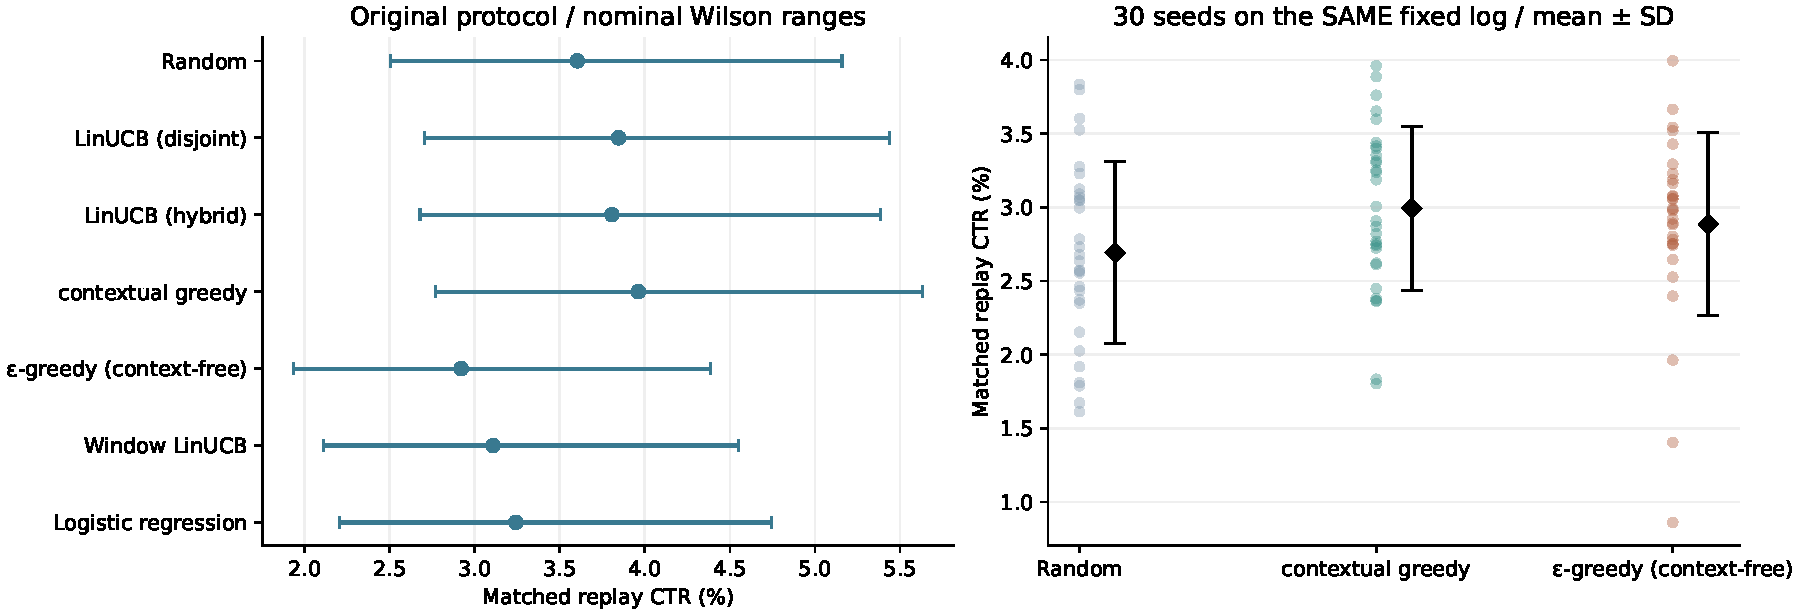
\includegraphics[width=\linewidth]{figures/yahoo_results.pdf}
\caption{Left: single-seed matched CTR with nominal Wilson ranges, which
omit selection uncertainty. Right: 30-seed CTRs for Random, contextual
greedy and context-free $\epsilon$-greedy; markers are mean $\pm$ SD, not a
population interval.}
\label{fig:yahoo}
\end{figure}

\subsection{Sparse-data diagnostic: fixed test, shrinking warmup}
Li et al. (2010, Table~1, Fig.~3) report hybrid's advantage in sparse
learning buckets and a larger pool. We hold the 15,786-event test fixed and
uniformly subsample the 84,214-event warmup to 100/10/5/1\% (seed 2026);
both LinUCB policies keep $\alpha=0.5$, so only warmup size changes
(Table~\ref{tab:sparse}).

\begin{table}[htbp]\centering\small\caption{Sparse warmup diagnostic on the fixed Yahoo test split. CTR is a matched-sample percentage; the last column is Hybrid minus Disjoint in percentage points.}\label{tab:sparse}\begin{tabular}{lrrrr}
\toprule
Warmup & Disjoint (m/clicks/CTR) & Hybrid (m/clicks/CTR) & H--D (pp) & Articles updated \\ \midrule
100\% & 780 / 30 / 3.846 & 788 / 30 / 3.807 & $-0.039$ & 21 \\
10\% & 738 / 21 / 2.846 & 782 / 20 / 2.558 & $-0.288$ & 21 \\
5\% & 736 / 19 / 2.582 & 786 / 21 / 2.672 & $+0.090$ & 21 \\
1\% & 781 / 25 / 3.201 & 784 / 21 / 2.679 & $-0.522$ & 20 \\
\bottomrule\end{tabular}\end{table}

Hybrid minus Disjoint is negative at three of four warmup levels and never
exceeds $+0.09$ pp: the paper's sparse-data advantage is not reproduced.
Warmup shrinkage reduces updated articles from 21 to 20 without helping
hybrid.

\begin{figure}[htbp]\centering
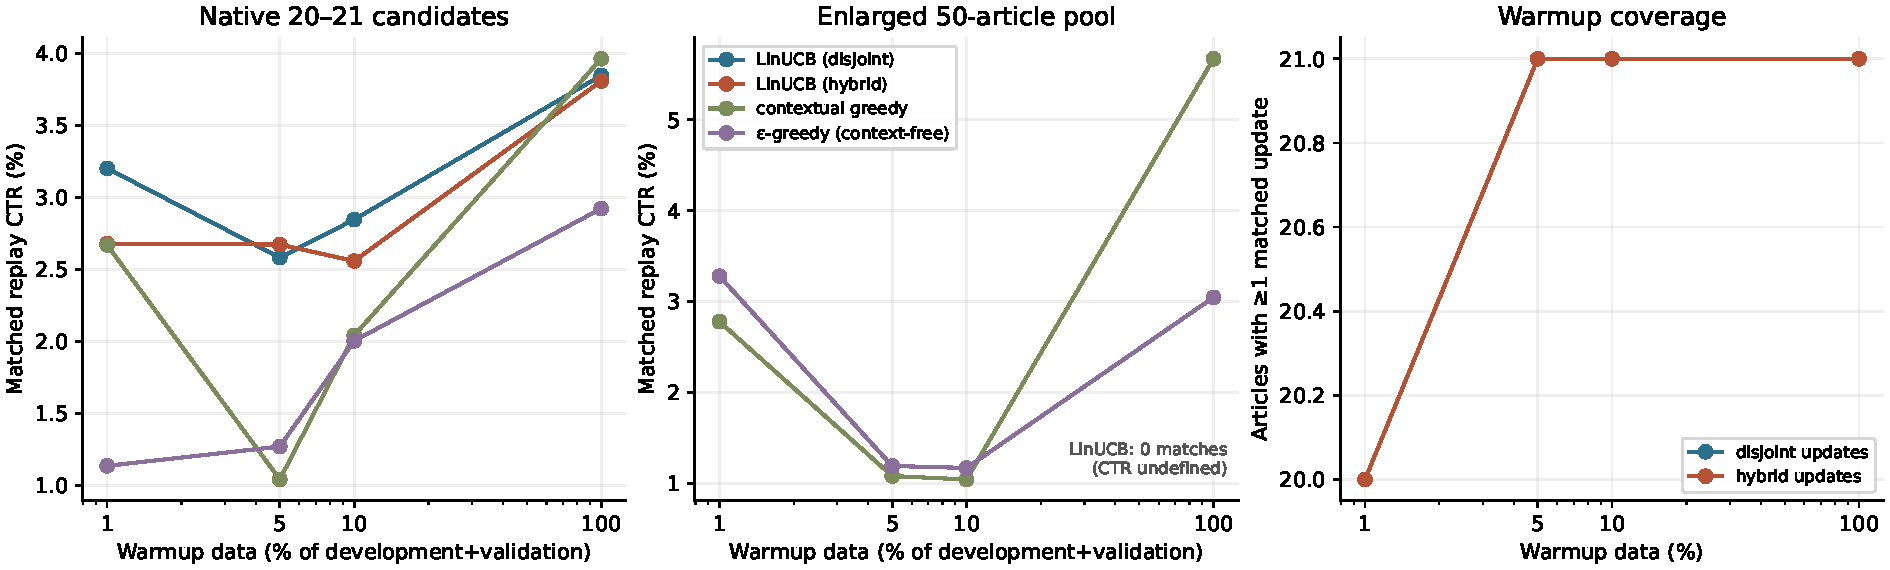
\includegraphics[width=\linewidth]{sparsity/sparsity.pdf}
\caption{Matched replay CTR versus warmup for the native and enlarged
pools (gaps: zero matches, undefined CTR); right: articles with an update.
The enlarged pool is a sensitivity check, not a faithful replay.}\label{fig:sparse}
\end{figure}

The enlarged pool is uninformative for deterministic LinUCB: both variants
have zero matched test events at every warmup level. With 50 candidates, no
exploration and a fixed tie-break they repeatedly pick articles the logger
never showed, so CTR is undefined (gaps in Fig.~\ref{fig:sparse}). The
stochastic greedy comparators do match, but are not comparable to the
native pool. This degeneracy is a further reason not to claim a deployment
gain from the enlarged pool.

\subsection{Supervised prediction and the OPE control}
Validation selects $C=10$ and threshold 0.060828. Test click prevalence is 2.661\%. AP is 0.0721, ROC-AUC 0.7373, log loss 0.1132, and Brier score 0.0253. At the validation threshold, precision is 0.0862, recall 0.3048 and F1 0.1344; the confusion matrix has TN=14,009, FP=1,357, FN=292 and TP=128. The threshold never uses test labels.

These metrics concern the logged click label, not LR's ranking of all
candidates or superiority over an adaptive bandit; a threshold is
unnecessary when ranking by probability, and classification and replay
answer different questions. The separate OPE check has 20,000 contexts,
four actions, a fixed target and a uniform logger with known $p=0.25$;
the independent reward model is constant 0.5. Oracle target mean is
0.538374, IPS 0.535600, SNIPS 0.539267, DR 0.539000. Agreement in one
realisation is a sanity check, not a variance or unbiasedness proof (SNIPS
remains finite-sample biased).

\subsection{Original preference-drift experiment}
\begin{table}[htbp]\centering\small\caption{Original poster study: mean $\pm$ sample SD of dynamic regret, 10 seeds per scenario.}\begin{tabular}{lrrr}
\toprule
Policy & Stationary & Abrupt & Gradual \\ \midrule
Random & 541.66 $\pm$ 4.48 & 542.77 $\pm$ 6.26 & 452.20 $\pm$ 5.26 \\
LinUCB (disjoint) & 191.06 $\pm$ 47.97 & 552.17 $\pm$ 8.67 & 461.00 $\pm$ 9.67 \\
Window LinUCB (300) & 165.53 $\pm$ 20.69 & 307.54 $\pm$ 31.94 & 235.12 $\pm$ 29.91 \\
\bottomrule\end{tabular}\end{table}

On the original generator the window reduces regret under both changes and
also in the stationary case. That stationary gain prevents attributing
everything to drift tracking: regularisation, the missing intercept and
scaling may matter. The negative Yahoo and positive simulation results
test different environments and evaluation units, so they do not conflict.

\begin{figure}[htbp]\centering
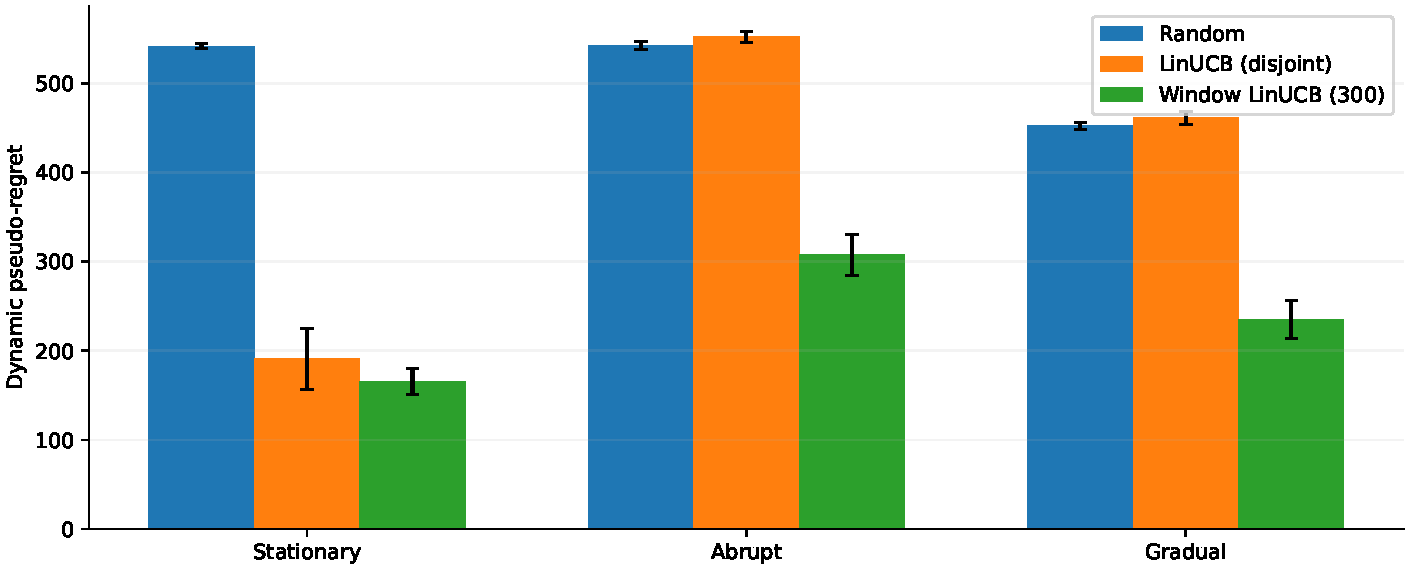
\includegraphics[width=.84\linewidth]{figures/poster_simulation.pdf}
\caption{Poster study: 3,000 rounds, seeds 0--9, $\alpha=0.25$, $W=300$;
bars are 95\% $t$ intervals. Only chosen-action feedback is observed.}
\label{fig:poster}
\end{figure}

\subsection{Independent seeds, intercept ablation and memory sensitivity}
\begin{table}[htbp]\centering\small\caption{Independent seeds 100--119: mean $\pm$ sample SD of regret, 20 worlds.}\begin{tabular}{lrrrr}
\toprule
Features & Policy & Stationary & Abrupt & Gradual \\ \midrule
original6 & LinUCB (disjoint) & 168.08 $\pm$ 38.66 & 554.29 $\pm$ 10.94 & 463.97 $\pm$ 8.95 \\
original6 & Window LinUCB (300) & 149.95 $\pm$ 22.64 & 285.91 $\pm$ 21.67 & 233.45 $\pm$ 25.30 \\
intercept7 & LinUCB (disjoint) & 156.18 $\pm$ 24.70 & 493.89 $\pm$ 34.53 & 415.19 $\pm$ 29.03 \\
intercept7 & Window LinUCB (300) & 227.58 $\pm$ 20.02 & 270.60 $\pm$ 20.62 & 223.17 $\pm$ 14.38 \\
\bottomrule\end{tabular}\end{table}

With six features, Window LinUCB (300) has stationary regret 149.95 versus
168.08 for LinUCB (disjoint), matching the poster direction. Adding the
intercept reverses that ordering (227.58 vs 156.18), yet with the
intercept the window still cuts abrupt regret 493.89 to 270.60 and gradual
regret 415.19 to 223.17. Adaptation gains survive this specification
check; the stationary benefit does not. The paired family intervals below
cover six declared contrasts, not every comparison or time point.

\begin{figure}[htbp]\centering
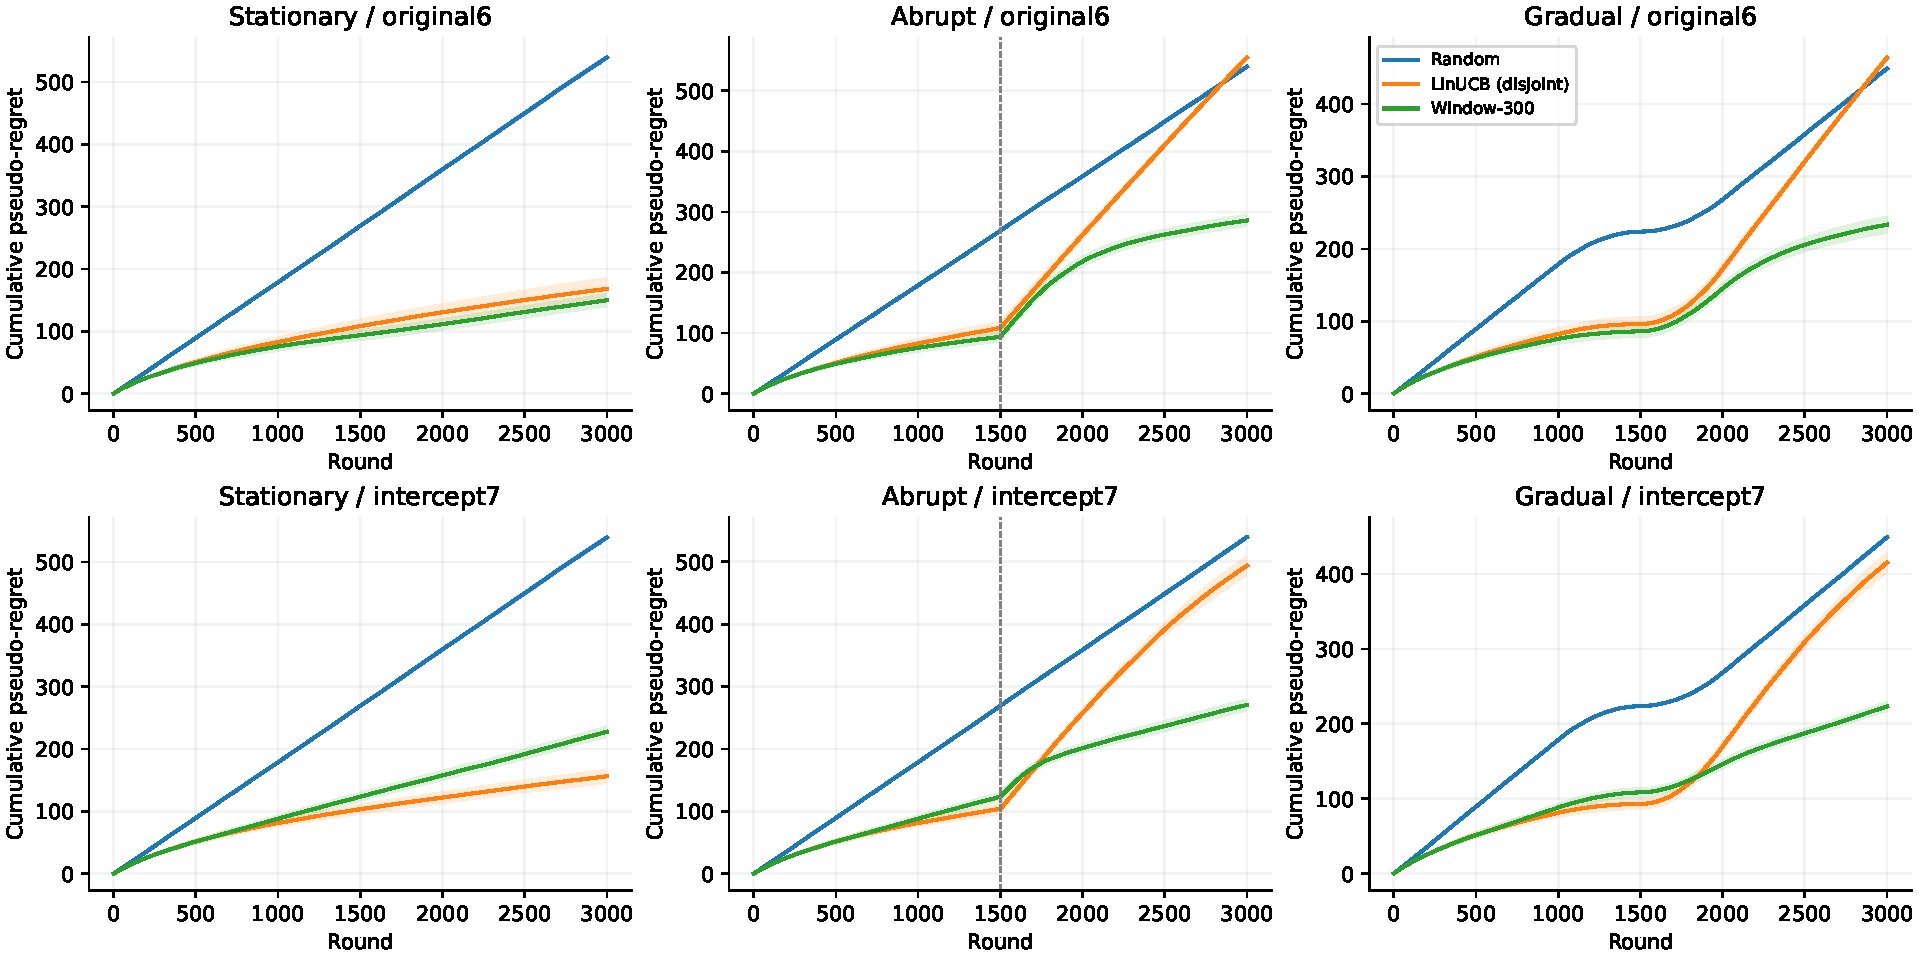
\includegraphics[width=\linewidth]{figures/replication_curves.pdf}
\caption{Seeds 100--119: upper row six features, lower row with intercept.
Lines are 20-world means, bands pointwise 95\% intervals; environments and
potential outcomes are paired.}
\label{fig:replicate}
\end{figure}

\begin{table}[htbp]\centering\small\caption{Window LinUCB (300) minus LinUCB (disjoint): paired differences and approximate 95\% family intervals adjusted for six contrasts. Negative favours the window.}\begin{tabular}{lrrr}
\toprule
Features & Scenario & Mean difference & Adjusted family interval \\ \midrule
original6 & stationary & -18.14 & [-35.41, -0.87] \\
original6 & abrupt & -268.38 & [-281.59, -255.17] \\
original6 & gradual & -230.52 & [-246.27, -214.78] \\
intercept7 & stationary & 71.40 & [59.92, 82.87] \\
intercept7 & abrupt & -223.29 & [-245.34, -201.23] \\
intercept7 & gradual & -192.02 & [-209.20, -174.84] \\
\bottomrule\end{tabular}\end{table}

For six features, Window-100/300/600 give stationary regrets
256.08/149.95/135.46, abrupt 280.13/285.91/409.91 and gradual
232.35/233.45/343.68: the long window keeps useful feedback but tracks
changes worse. The intercept-feature sensitivity has its own
ordering; these are descriptive, not test-selected, windows. The
contextual-greedy control also shows stale-data bias (555.68 abrupt,
464.64 gradual, six features). No multiplicity-adjusted claim is made for
these additional comparisons.

\begin{figure}[htbp]\centering
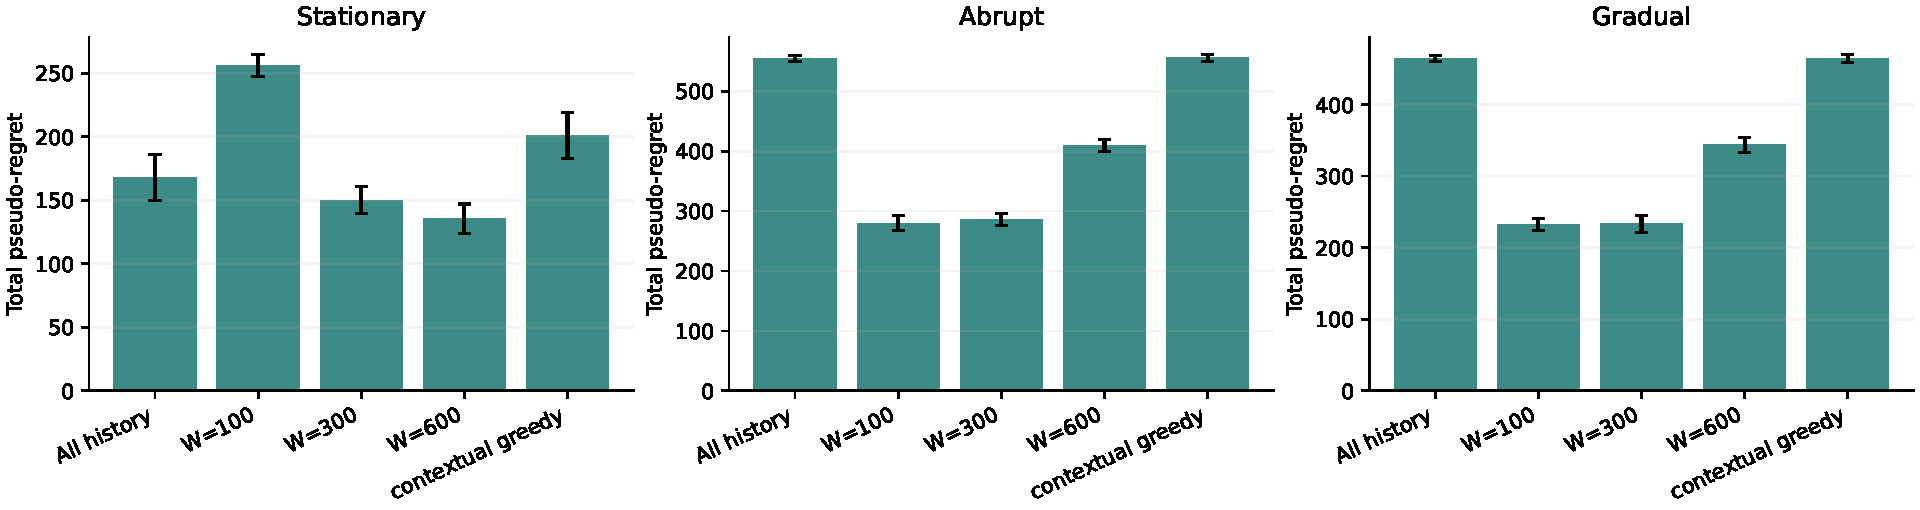
\includegraphics[width=\linewidth]{figures/window_ablation.pdf}
\caption{Six-feature window sensitivity and contextual-greedy control on
seeds 100--119: mean total regret with pointwise 95\% intervals. The fixed
grid is a sensitivity study, not test-world tuning.}
\label{fig:window}
\end{figure}

\section{Discussion: strengths, limits and interpretation}
\textbf{Strengths.} The two parts answer complementary questions rather
than substituting simulation for logged data. Both Li et al. 2010
estimators are checked against closed forms; the replay, drift study and
extension are fully specified and reproducible in a frozen environment.
Feedback visibility, selection, seeds and interval scope are documented,
and the unfavourable Yahoo window result is retained without fabricating
counterfactual labels or propensities.

\textbf{Limits.} Yahoo covers 80 minutes with small matched samples; the
logger and candidate construction need further verification for
policy-value identification. Test bandits adapt while LR is frozen, with
different features and budgets. Anonymous profiles are not verified user
IDs, and file hashes do not validate article-vector semantics. The
simulator omits arrivals, delayed clicks, position effects and returning
users; its sign reversal is simple and its original six-feature map
misspecified. The intercept ablation does not isolate one causal reason.
Twenty worlds and a small grid cannot establish a universal memory rule.
Hybrid assumes the decomposition of Eq.~\eqref{eq:hybridmean}; uninformative
article features let its extra variance offset sharing. The sparse
diagnostic cannot recreate the paper's sparse buckets from an 80-minute
log, and the enlarged pool is not a valid replay for non-exploring LinUCB.

\textbf{Practical meaning.} The project evaluates forgetting; a
synthetic improvement alone does not justify deployment. Recent feedback
helps in some controlled changes, while Yahoo leaves the real benefit
unresolved. A longer, correctly logged dataset and a predeclared
deployment evaluation are needed for any news-CTR claim.

\section{Conclusion and concrete extensions}
The plan is realised as chronological Yahoo replay plus known-mean drift
experiments. Seven policies include faithful LinUCB (disjoint) and LinUCB
(hybrid) and the paper's context-free $\epsilon$-greedy; neither hybrid nor
window wins on the held-out log, and the sparse-warmup diagnostic does not
reproduce the hybrid benefit. Simulations favour the window under specified
changes, and an intercept/window study tests robustness without changing
the task. The conclusion is conditional: forgetting helps the tested drift
worlds, but offline CTR and simulated regret do not establish online gain.

\textbf{Theory.} Bound the stale-data term in Eq.~\eqref{eq:drift} under
variation and support assumptions, separating tracking, noise and
misspecification; address Faury et al. \cite{faury2021} rather than reusing
a stationary guarantee. A sharper radius for Eq.~\eqref{eq:hybridvar} is
open. \textbf{Algorithm.} Compare windows with discounted/restarted variants
on independent streams; add cold starts, time-varying $\beta$ and low-rank
article embeddings. \textbf{Application.} Obtain longer logs with known
candidate support, genuine user IDs and propensities, then use a
predeclared off-policy or online design. MIND/Adressa demos and NeuralUCB
remain extensions, not completed claims.

\section*{Reproducibility and AI assistance}
The package has source, fourteen tests, core and seed results, the
sparsity diagnostic and plotting/audit code. \texttt{./run.sh} runs every
stage with \texttt{uv run --frozen}; \texttt{./build\_report.sh} recompiles
the PDFs and \texttt{verify\_consistency.py} audits numbers, hashes, pages
and review freshness. No network is needed once Python 3.13.2 and the
lockfile are present; hashes and exact versions are in Appendix A and JSON
manifests. The project is CPU-only; no GPU or API key is needed. AI tools assisted
drafting, derivation review and supplementary analysis; all numbers come
from included programs. Assistance does not turn replay into an online
experiment.

\begin{thebibliography}{9}\footnotesize\setlength{\itemsep}{2pt}\setlength{\parskip}{0pt}
\bibitem{li2010} L. Li, W. Chu, J. Langford, and R. E. Schapire.
A Contextual-Bandit Approach to Personalized News Article Recommendation.
\emph{WWW}, 2010. \url{https://arxiv.org/abs/1003.0146}.
\bibitem{li2011} L. Li, W. Chu, J. Langford, and X. Wang.
Unbiased Offline Evaluation of Contextual-bandit-based News Article
Recommendation Algorithms. \emph{WSDM}, 2011. \url{https://arxiv.org/abs/1003.5956}.
\bibitem{cheung2019} W. C. Cheung, D. Simchi-Levi, and R. Zhu.
Learning to Optimize under Non-Stationarity. \emph{AISTATS}, PMLR
89:1079--1087, 2019. \url{https://proceedings.mlr.press/v89/cheung19b.html}.
\bibitem{russac2019} Y. Russac, C. Vernade, and O. Cappe.
Weighted Linear Bandits for Non-Stationary Environments.
\emph{NeurIPS} 32, 2019. \url{https://proceedings.neurips.cc/paper/2019/hash/263fc48aae39f219b4c71d9d4bb4aed2-Abstract.html}.
\bibitem{zhao2020} P. Zhao, L. Zhang, Y. Jiang, and Z.-H. Zhou.
A Simple Approach for Non-stationary Linear Bandits. \emph{AISTATS},
PMLR 108:746--755, 2020. \url{https://proceedings.mlr.press/v108/zhao20a.html}.
\bibitem{faury2021} L. Faury, Y. Russac, M. Abeille, and C. Calauzenes.
A Technical Note on Non-Stationary Parametric Bandits: Existing Mistakes
and Preliminary Solutions. \emph{ALT}, PMLR 132:619--626, 2021.
\url{https://proceedings.mlr.press/v132/faury21a.html}.
\bibitem{dudik2011} M. Dudik, J. Langford, and L. Li.
Doubly Robust Policy Evaluation and Learning. \emph{ICML}, 2011.
\url{https://arxiv.org/abs/1103.4601}.
\end{thebibliography}

\clearpage\appendix
\section{Data and execution manifest}
\begin{center}\small\begin{tabular}{lr}
\toprule
Field & Executed value \\ \midrule
Yahoo events / articles / span & 100,000 / 80 / 4,800 seconds \\
Development / validation / test & 66,204 / 18,010 / 15,786 \\
Logged action in candidate set & True \\
Unique candidates per event & True \\
Core stochastic seed / seed sweep & 2026 / 2026--2055 \\
Original / independent simulation seeds & 0--9 / 100--119 \\
Simulation horizon / candidates & 3,000 / 6 \\
Independent configurations / trajectories & 12 / 720 \\
Python (locked) & 3.13.2 \\
NumPy / SciPy & 2.4.3 / 1.17.1 \\
scikit-learn / matplotlib / joblib & 1.8.0 / 3.10.8 / 1.5.3 \\
\bottomrule\end{tabular}\end{center}

\noindent Environment locking. \texttt{pyproject.toml} pins Python 3.13.2
and exact versions, \texttt{uv.lock} records wheel URLs and SHA-256, and
\texttt{.python-version} selects the interpreter. \texttt{run.sh} fixes
\texttt{OPENBLAS\_NUM\_THREADS=1}, \texttt{OMP\_NUM\_THREADS=1},
\texttt{MKL\_NUM\_THREADS=1}, \texttt{OPENBLAS\_CORETYPE=Haswell} and
\texttt{PYTHONHASHSEED=0}, then uses \texttt{uv run --frozen}; on x86-64
this fixes the numerical path.

\noindent Yahoo log SHA-256:
\begin{quote}\footnotesize\url{45a5ce2a1f64875389d5a5bcc65be8e95c3b6a91b53757e90b055da49915525f}\end{quote}
\noindent Article file SHA-256:
\begin{quote}\footnotesize\url{07404caa43916d8b5e942a5016065222cec2e8ac44a57580cd584568d8232f9e}\end{quote}
\noindent Experiment source SHA-256:
\begin{quote}\footnotesize\url{03d683671b15965dffc1a5ad15dfcd4864e370857fb6de1c45702c962e5956eb}\end{quote}
\noindent Extension source SHA-256:
\begin{quote}\footnotesize\url{524c89fe65acf80d69140547ff324e0f77110668df715710cd37549754c818ac}\end{quote}
\noindent Sparsity source SHA-256:
\begin{quote}\footnotesize\url{6dbcb5ec4f43bab54f3e74804ed8f37752c580c4a9a8a51822b0346582c859bf}\end{quote}

Raw Yahoo files under \texttt{reproduction/Yahoo\_recommendation/data/}
match these hashes; derived figures need no external data. All values are
regenerated by the locked pipeline, not copied from a prior run.

The complete window and feature-map sensitivity table is in
\texttt{robustness/results.json}.

\end{document}
